% Variational autoencoder -- subsection of "Encoding", pulled in by sections/05-encoding.tex.
% Red \TODO{...} marks replace the [square-bracket] placeholders of the original draft.

\subsection[Variational autoencoder]{Variational Autoencoder for Airway Tree Representation Learning}
\label{sec:vae}                          % \secref{sec:vae}

% ------------------------------------------------------------------------------
\subsubsection{Motivation}               % why a VAE is used
\label{sec:vae_motivation}               % \secref{sec:vae_motivation}

To learn a compact representation of airway trees, we represent each tree as a binary
voxel occupancy grid. As \citet{brock2016} point out, there is no meaningful way
to interpolate directly between two binary grids. Relating voxelized shapes to one another
therefore requires a model that works in an abstract feature space capturing the main
factors of variation.

For this reason we use a Variational Autoencoder (VAE) \cite{kingma2014}. A VAE is a
probabilistic framework that learns two networks jointly:
\begin{itemize}                          % the two VAE components
  \item an \textbf{inference (encoder) network}, which maps an input to a set of latent
        variables describing it, and
  \item a \textbf{generative (decoder) network}, which maps from the latent space back to
        the input space.
\end{itemize}

Once the encoder has learned latent variables that describe the underlying variation between
shapes, each airway tree can be encoded as a latent vector. That vector can be used as a
learned representation, or interpolated and decoded back into a voxel grid. Our models
are adapted from the voxel-based VAE of \citet{brock2016}.

% ------------------------------------------------------------------------------
\subsubsection{Model architecture}       % encoder, latent layer, decoder for both resolutions
\label{sec:vae_architecture}             % \secref{sec:vae_architecture}

\paragraph{Input resolutions.}           % the two voxel grids used
Each airway tree was voxelized into a binary occupancy grid at two resolutions,
$128\times128\times128$ and $256\times256\times256$ voxels. The higher resolution preserves
more of the thin distal branches, at the cost of a much larger memory and computational
footprint. We trained a separate VAE for each resolution. Both networks follow the design
principles of \citet{brock2016}, adapted to the larger input size. The
$256^3$ model has one additional downsampling stage (two extra encoder layers), so that both
networks reach the same $7\times7\times7$ spatial grid at the bottleneck. The architectures
are summarized in Figure~\ref{fig:vae_arch} and Table~\ref{tab:vae_layers}.

\paragraph{Encoder.}                     % conv blocks, strided downsampling, channel growth
The encoder is a stack of 3D convolutional blocks. Each block consists of a
$3\times3\times3$ convolution without bias, instance normalization with learnable affine
parameters, and an ELU activation. As in \citet{brock2016}, downsampling is
performed with strided convolutions rather than pooling, in every second layer. The layers
alternate between an unpadded stride-1 convolution, which reduces each spatial dimension by
2, and a stride-2 convolution with padding 1, which approximately halves it. The number of
filters doubles at every layer:
\begin{itemize}                          % per-resolution encoder details
  \item \textbf{$128^3$ model:} 8 convolutional layers, starting with 2 filters and reaching
        256 filters. The spatial size goes
        $128 \to 126 \to 63 \to 61 \to 31 \to 29 \to 15 \to 13 \to 7$.
  \item \textbf{$256^3$ model:} 10 convolutional layers, starting with 4 filters and reaching
        2048 filters. The spatial size goes
        $256 \to 254 \to 127 \to 125 \to 63 \to 61 \to 31 \to 29 \to 15 \to 13 \to 7$.
\end{itemize}
A $1\times1\times1$ convolution (followed by instance normalization and ELU) then reduces the
number of channels to 32 while keeping the $7^3$ grid. The result is flattened into a vector
of $32 \cdot 7^3 = 10{,}976$ features. In \citet{brock2016}, a fully connected
layer is placed between the convolutional features and the latent projection. In our models
this layer is removed, and the flattened features are mapped directly by two separate linear
layers to the mean $\boldsymbol{\mu}$ and the log standard deviation $\log\boldsymbol{\sigma}$
of the latent Gaussian, of dimension \TODO{100}. The log standard deviation is clamped to
$[-10, 10]$ for numerical stability.

\paragraph{Latent sampling.}             % reparameterization during training vs. inference
During training, a latent vector is sampled with the reparameterization
trick \cite{kingma2014},
\begin{equation}
  \mathbf{z} = \boldsymbol{\mu} + \exp(\log\boldsymbol{\sigma}) \odot \boldsymbol{\epsilon},
  \qquad \boldsymbol{\epsilon} \sim \mathcal{N}(\mathbf{0}, \mathbf{I}).
  \label{eq:reparam}                     % reparameterization with log-sigma parameterization
\end{equation}
At inference time the mean is used directly ($\mathbf{z} = \boldsymbol{\mu}$), giving a
deterministic encoding of each airway tree.

\paragraph{Decoder.}                     % mirrored decoder with resize-convolution upsampling
The decoder mirrors the encoder, and its weights are not tied to the encoder's. A linear
layer maps $\mathbf{z}$ back to 10,976 features, followed by layer
normalization \cite{ba2016} and ELU, and the result is reshaped into a $32\times7^3$ volume.
A stride-1 convolutional block expands the channels to the width of the deepest encoder layer
(256 for the $128^3$ model, 2048 for the $256^3$ model). The decoder then alternates between
upsampling blocks and stride-1 convolutional blocks (padding 1, spatial size preserved),
halving the number of channels at every layer.

\citet{brock2016} upsample with fractionally strided (transposed) convolutions.
We instead use a resize-convolution: each upsampling block applies nearest-neighbour
upsampling to an exact target size, followed by a $3\times3\times3$ convolution, instance
normalization and ELU. This avoids the checkerboard artifacts associated with transposed
convolutions \cite{odena2016} and lets the decoder match the odd intermediate sizes of the
encoder (15, 31, 63, 127) exactly. The spatial size goes
$7 \to 15 \to 31 \to 63 \to 128$ for the $128^3$ model and
$7 \to 15 \to 31 \to 63 \to 127 \to 256$ for the $256^3$ model.

A final $3\times3\times3$ convolution with bias maps the features to a single output channel,
with no normalization or activation. Its outputs are logits; the sigmoid applied inside the
loss converts them into the predicted probability that each voxel is occupied.

\paragraph{Normalization, activations and initialization.}  % departures from the original
All layers use the ELU activation \cite{clevert2016}, except the output layer. Where Brock et
al.\ use Batch Normalization \cite{ioffe2015}, we use instance
normalization \cite{ulyanov2016}. At $128^3$ and $256^3$ resolution, GPU memory limits the
batch size to a few samples, which makes batch statistics unreliable; instance normalization
normalizes each sample independently and does not depend on batch size. Convolutional and
linear weights are initialized with Glorot (Xavier) normal initialization \cite{glorot2010},
and biases are initialized to zero.

\begin{table}[htbp]                      % layer-by-layer summary of both models
  \centering                             % center the table
  \small                                 % slightly smaller font so the table fits
  \caption{Summary of the two VAE architectures.}
  \label{tab:vae_layers}                 % referenced as Table~\ref{tab:vae_layers}
  \begin{tabular}{lcc}                   % 3 columns: stage, 128 model, 256 model
    \toprule
    Stage & $128^3$ model & $256^3$ model \\
    \midrule
    Input & $1 \times 128^3$ & $1 \times 256^3$ \\
    Encoder conv layers & 8 & 10 \\
    Filters (first $\to$ last) & $2 \to 256$ & $4 \to 2048$ \\
    Encoder output & $256 \times 7^3$ & $2048 \times 7^3$ \\
    $1\times1\times1$ reduction & $32 \times 7^3$ & $32 \times 7^3$ \\
    Flattened features & 10,976 & 10,976 \\
    Latent dimension & \TODO{100} & \TODO{100} \\
    Decoder upsampling steps & 4 & 5 \\
    Decoder filters (first $\to$ last) & $256 \to 2$ & $2048 \to 4$ \\
    Output & $1 \times 128^3$ (logits) & $1 \times 256^3$ (logits) \\
    \bottomrule
  \end{tabular}
\end{table}

\begin{figure}[htbp]                     % placeholder for the architecture diagram
  \centering                             % center the figure
  % 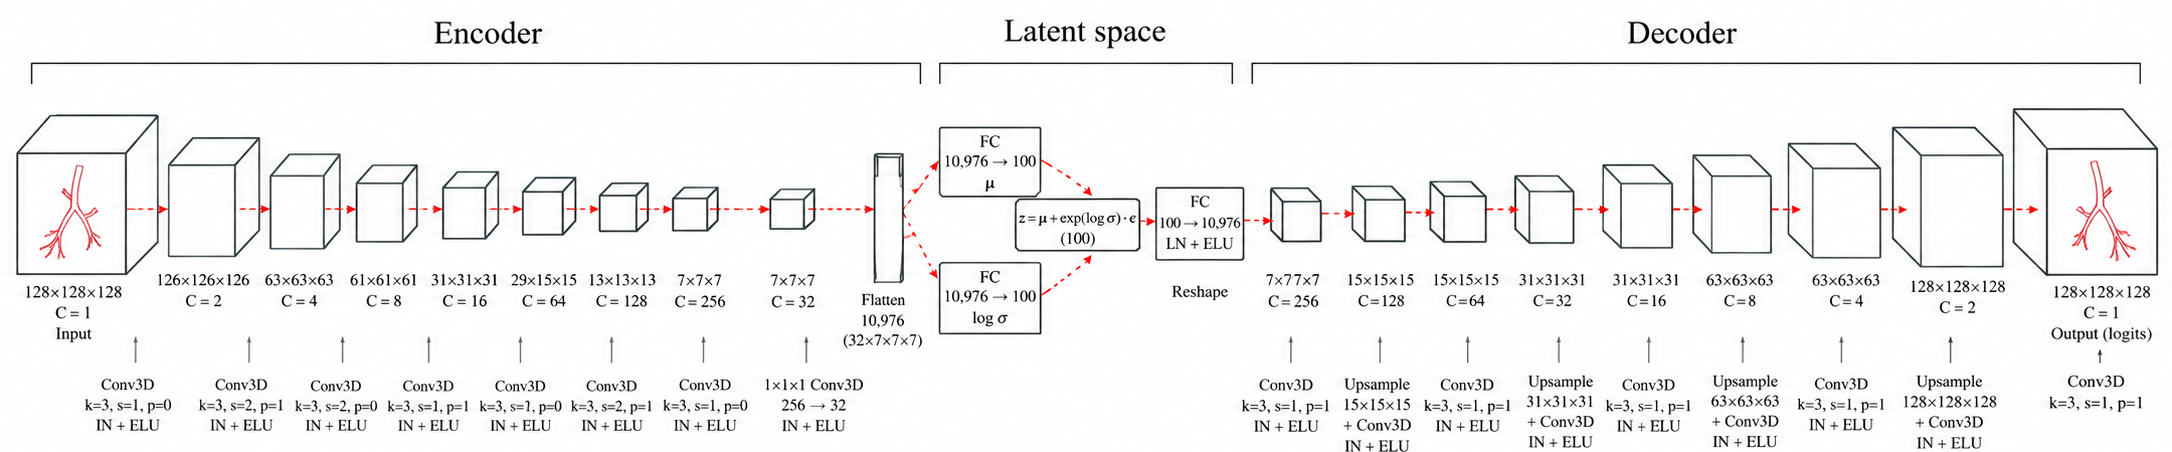
\includegraphics[width=\textwidth]{figures/vae_architecture.png}  % uncomment with your file
  \fbox{\parbox[c][4cm][c]{0.9\textwidth}{\centering [VAE architecture figure]}}  % remove once image added
  \caption{Architecture of the voxel-based VAEs, adapted from \citet{brock2016}. Shown for
           the $256^3$ model; the $128^3$ model omits the first downsampling stage.}
  \label{fig:vae_arch}                   % referenced as Figure~\ref{fig:vae_arch}
\end{figure}

% ------------------------------------------------------------------------------
\subsubsection{Loss function}            % BCE modification, KL, L2, clDice
\label{sec:vae_loss}                     % \secref{sec:vae_loss}

Following \citet{brock2016}, the loss combines three terms: the KL divergence
between the approximate posterior and the prior on the latent variables, L2 weight
regularization, and a reconstruction term based on a modified Binary Cross-Entropy (BCE).
We then add a fourth term, clDice, described below.

\paragraph{Modified BCE.}                % why and how the BCE is modified
The standard BCE is
\begin{equation}
  \mathcal{L}_{\mathrm{BCE}} = -t\log(o) - (1-t)\log(1-o),
  \label{eq:bce}                         % standard binary cross-entropy
\end{equation}
where $t \in \{0,1\}$ is the target voxel value and $o \in (0,1)$ is the network output.
\citet{brock2016} identify two problems with this loss for voxel data. First, its
derivative with respect to $o$ becomes very small as $o$ approaches $t$, which can cause
vanishing gradients. Second, it penalizes false positives and false negatives equally. Most
of a voxel grid is empty, so the network can fall into a poor local optimum by predicting
every voxel as empty. The second problem is even more severe for airway trees than for the
ModelNet objects in the original paper: airways are thin, branching structures that occupy a
very small fraction of the grid.

\citet{brock2016} propose two modifications to address these problems: shifting
the target and output ranges to increase the gradient magnitude, and weighting false negatives
against false positives. In our implementation we adopt the second modification. The targets
remain binary, $t \in \{0,1\}$, and the output $o$ is the sigmoid of the decoder logits,
clamped to $[\epsilon, 1-\epsilon]$ with $\epsilon = 10^{-7}$ to avoid $\log(0)$. A
hyperparameter $\gamma$ weights false negatives against false positives:
\begin{equation}
  \mathcal{L}_{\mathrm{BCE\text{-}mod}} = -\gamma\, t\log(o) - (1-\gamma)(1-t)\log(1-o).
  \label{eq:bce_mod}                     % gamma-weighted BCE from Brock et al.
\end{equation}
The loss is summed over all voxels of a sample and averaged over the batch. We set
$\gamma = \TODO{0.99}$, which strongly penalizes missed voxels and reduces the penalty for
spurious ones; this is slightly higher than the $0.97$ used by Brock et al., reflecting the
even stronger class imbalance of airway trees. Brock et al.\ report that a $\gamma$ that is too
high gives noisy reconstructions, while a $\gamma$ that is too low gives reconstructions that
lose important structural details.

\paragraph{KL term.}                     % beta-VAE weighting and L2 via weight decay
The KL divergence is summed over the latent dimensions and averaged over the batch, and it is
weighted by a factor $\beta$, following the $\beta$-VAE formulation \cite{higgins2017}.
L2 weight regularization is applied through the optimizer's weight decay, with coefficient
\TODO{value}.

\paragraph{clDice (our addition).}       % topology-preserving term added on top
Voxel-wise losses do not explicitly preserve the connectivity of tubular structures, which is
essential for airway trees. We therefore add the centerline Dice (clDice)
loss \cite{shit2021} to the reconstruction objective. Let $V_P$ and $V_L$ be the predicted
and ground-truth volumes, and $S_P$ and $S_L$ their soft skeletons. clDice is defined as
\begin{equation}
  T_{\mathrm{prec}} = \frac{|S_P \cap V_L|}{|S_P|}, \qquad
  T_{\mathrm{sens}} = \frac{|S_L \cap V_P|}{|S_L|},
  \label{eq:tprec_tsens}                 % topology precision and sensitivity
\end{equation}
\begin{equation}
  \mathrm{clDice} = 2\,\frac{T_{\mathrm{prec}} \cdot T_{\mathrm{sens}}}
                             {T_{\mathrm{prec}} + T_{\mathrm{sens}}}.
  \label{eq:cldice}                      % harmonic mean of the two
\end{equation}
Topology precision is the fraction of the predicted skeleton lying inside the ground-truth
volume, and topology sensitivity is the fraction of the ground-truth skeleton lying inside
the predicted volume. The final training objective is
\begin{equation}
  \mathcal{L}_{\mathrm{total}} = \mathcal{L}_{\mathrm{BCE\text{-}mod}}
  + \beta\,\mathcal{L}_{\mathrm{KL}}
  + \lambda\,(1 - \mathrm{clDice})
  + \mathcal{L}_{\mathrm{L2}},
  \label{eq:total_loss}                  % full training loss
\end{equation}
with $\beta = \TODO{value}$ and $\lambda = \TODO{value}$.

% ------------------------------------------------------------------------------
\subsubsection{Training}                 % optimizer, learning rate, data split
\label{sec:vae_training}                 % \secref{sec:vae_training}

The model is trained with stochastic gradient descent using Nesterov
momentum \cite{sutskever2013}. Training runs for up to \TODO{100} epochs, or until the
reconstruction error on a held-out validation set stops decreasing. Following
\citet{brock2016}, the learning rate is \TODO{0.0001} for the first epoch and then raised to
\TODO{0.001}. The dataset contains \TODO{N} airway trees, split into
\TODO{$N_{\mathrm{train}}$} training, \TODO{$N_{\mathrm{val}}$} validation and
\TODO{$N_{\mathrm{test}}$} test samples. Training used a batch size of \TODO{batch size} on
\TODO{GPU}.

% ------------------------------------------------------------------------------
\subsubsection{Results}                  % training vs. validation behaviour
\label{sec:vae_results}                  % \secref{sec:vae_results}

During training, the reconstruction loss on the training set decreased steadily, and the
model reconstructed training airway trees well. Performance on held-out data was much worse.
The validation loss did not follow the training loss (Figure~\ref{fig:vae_curves}).
Reconstructions of validation and test trees were poor, with \TODO{e.g.\ missing branches,
broken connectivity, blurred or blob-like structures} (Figure~\ref{fig:vae_recon}).

This gap between training and validation performance shows that the model
\textbf{overfits}: it memorizes the training samples instead of learning a representation
that generalizes to unseen airway trees.

\citet{brock2016} observed a relevant limitation of their own voxel VAE. It
struggled to reconstruct objects with long, thin parts, such as table and chair legs. The
authors suggest that such small features contribute little to the global loss and get lost in
favor of denser regions. They also note that the VAE tends to produce smooth, rounded outputs
rather than sharp edges. Airway trees consist almost entirely of thin, branching tubes, so this
limitation likely contributes to the poor reconstructions we observed, even with the added
clDice term.

\begin{figure}[htbp]                     % placeholder for training/validation curves
  \centering                             % center the figure
  % 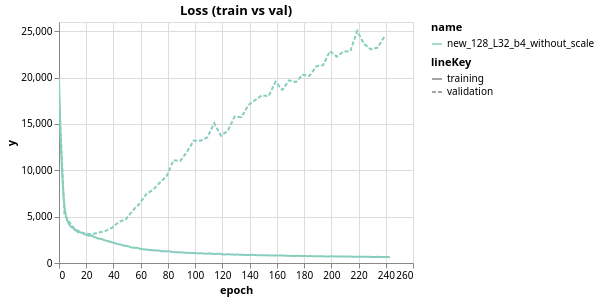
\includegraphics[width=\textwidth]{figures/vae_training_curves.png}  % uncomment with your file
  \fbox{\parbox[c][4cm][c]{0.9\textwidth}{\centering [Training and validation loss curves]}}
  \caption{Training and validation losses of the VAE. The validation loss does not follow
           the decrease of the training loss, indicating overfitting.}
  \label{fig:vae_curves}                 % referenced as Figure~\ref{fig:vae_curves}
\end{figure}

\begin{figure}[htbp]                     % placeholder for reconstruction examples
  \centering                             % center the figure
  % 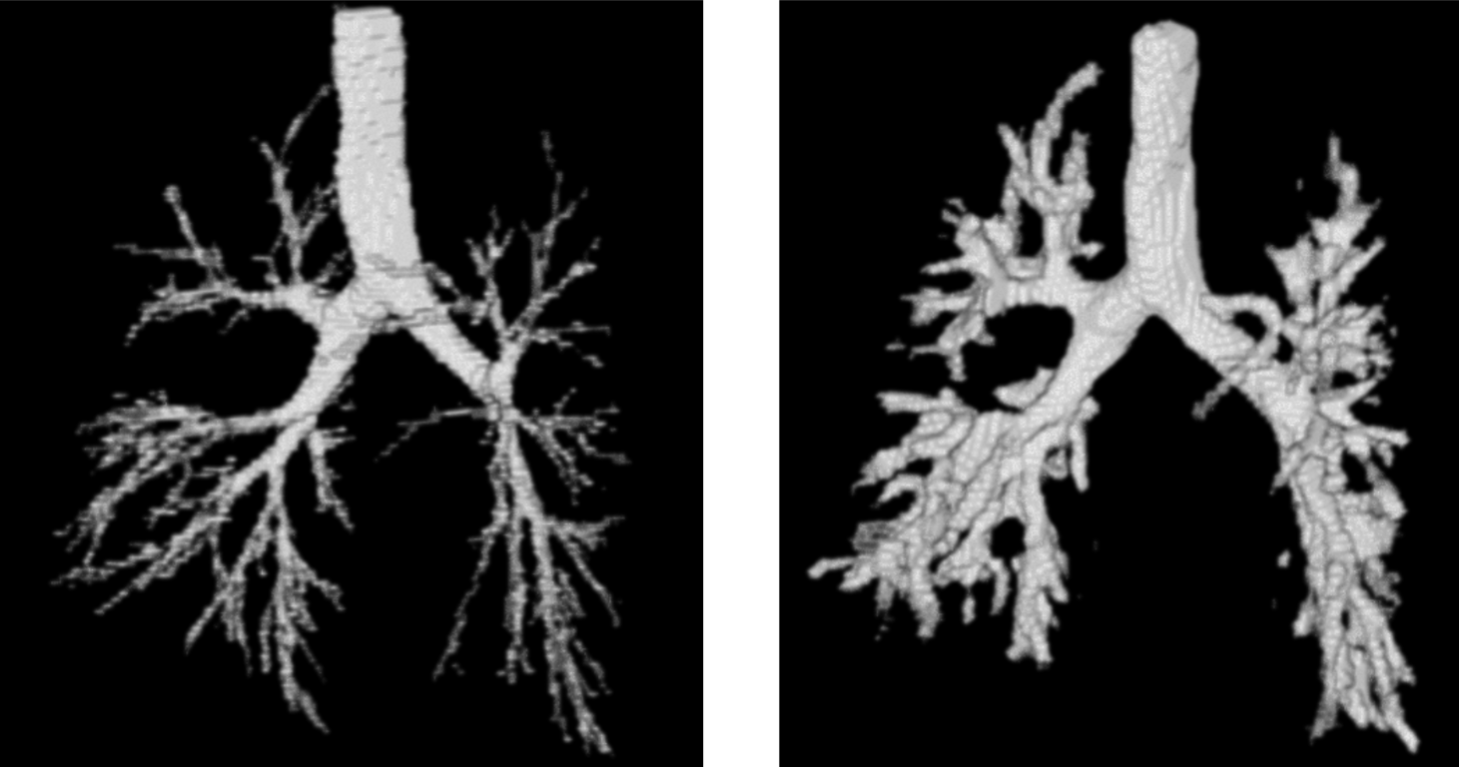
\includegraphics[width=\textwidth]{figures/vae_reconstructions.png}  % uncomment with your file
  \fbox{\parbox[c][4cm][c]{0.9\textwidth}{\centering [Original vs.\ reconstructed airway trees]}}
  \caption{Original airway trees and their VAE reconstructions for training (top) and
           validation/test (bottom) samples.}
  \label{fig:vae_recon}                  % referenced as Figure~\ref{fig:vae_recon}
\end{figure}

% ------------------------------------------------------------------------------
\subsubsection{Mitigating overfitting}   % augmentation and dropout attempts
\label{sec:vae_overfitting}              % \secref{sec:vae_overfitting}

To reduce overfitting, we applied two regularization strategies.

\paragraph{Data augmentation.}           % first regularization strategy
Each training sample was randomly transformed with \TODO{random translations, flips,
rotations, small elastic deformations, noise}. This increases the effective size and
variability of the training set. \citet{brock2016} use a similar strategy, training on both a
corrupted and an uncorrupted copy of each instance so that the network learns invariance to
small structural variations.

\paragraph{Dropout.}                     % second regularization strategy
Dropout layers with rate \TODO{$p$} were added to \TODO{the fully connected layers / the
encoder / the decoder} to discourage co-adaptation of features.

Neither strategy resolved the problem. As shown in Figure~\ref{fig:vae_curves_reg}, the
training and validation curves still diverge after adding augmentation and dropout, and
validation and test reconstructions remain poor. This suggests the limitation lies deeper than
a lack of regularization. Plausible causes include the small size of the dataset relative to
model capacity, the low voxel resolution relative to the thinness of the airway branches, and
the difficulty voxel VAEs have with thin structures.

\begin{figure}[htbp]                     % placeholder for curves after regularization
  \centering                             % center the figure
  % \includegraphics[width=\textwidth]{figures/vae_curves_regularized.png}  % uncomment with your file
  \fbox{\parbox[c][4cm][c]{0.9\textwidth}{\centering [Loss curves with augmentation and dropout]}}
  \caption{Training and validation losses after adding data augmentation and dropout. The
           gap between training and validation performance persists.}
  \label{fig:vae_curves_reg}             % referenced as Figure~\ref{fig:vae_curves_reg}
\end{figure}
